% Created 2015-03-19 Thu 18:28
\documentclass[11pt]{article}
\usepackage[utf8]{inputenc}
\usepackage{lmodern}
\usepackage[T1]{fontenc}
\usepackage{fixltx2e}
\usepackage{graphicx}
\usepackage{longtable}
\usepackage{float}
\usepackage{wrapfig}
\usepackage{rotating}
\usepackage[normalem]{ulem}
\usepackage{amsmath}
\usepackage{textcomp}
\usepackage{marvosym}
\usepackage{wasysym}
\usepackage{amssymb}
\usepackage{amsmath}
\usepackage[version=3]{mhchem}
\usepackage[numbers,super,sort&compress]{natbib}
\usepackage{natmove}
\usepackage{url}
\usepackage{minted}
\usepackage{underscore}
\usepackage[linktocpage,pdfstartview=FitH,colorlinks,
linkcolor=blue,anchorcolor=blue,
citecolor=blue,filecolor=blue,menucolor=blue,urlcolor=blue]{hyperref}
\usepackage{attachfile}
\usepackage[left=1in, right=1in, top=1in, bottom=1in, nohead]{geometry}
\usepackage{hyperref}
\usepackage{setspace}
\usepackage[labelfont=bf]{caption}
\usepackage{amsmath}
\usepackage{enumerate}
\usepackage[parfill]{parskip}
\author{Prateek Mehta, William F. Schneider}
\date{03-05-2015 Thu}
\title{Computational Chemistry Laboratory III (CBE 60547)}
\begin{document}

\maketitle


\section{A review of what we know}
\label{sec-1}

So far we have learned how to:

\begin{itemize}
\item navigate the linux terminal

\item create create and edit files using Emacs

\item numerical analysis and plotting with Python

\item different concepts in molecular simulations, e.g. potential energy surfaces, geometry optimizations, etc.
\end{itemize}

It might make sense to go back and read the lecture notes and notes from Lab 1 and Lab 2 if you feel the need to re-familiarize yourself with these things. In this lab, we will combine some of the things we learned and to perform DFT calculations with a powerful software package, \texttt{VASP}. 


\section{Loading the required software}
\label{sec-2}

Before we can actually proceed, we will need to tell our computer how it can find all the tools we need. We will store this information so that the software is already loaded for us every time we login in the future. Depending on your unix shell, the things we need to do will be a little different. You can see which shell you are using with the command \verb~echo $0~. 

The software we need is dependent on the bash shell and thus we (all users) need to add a few commands to our \verb~.bashrc~ file. Go to your home directory and open the \texttt{.bashrc} file, i.e., run the following two commands. 

\begin{minted}[frame=lines,fontsize=\scriptsize,linenos]{sh}
cd
emacs .bashrc
\end{minted}

Once there, add the following line at the bottom of the file and save it (Make sure there are no typos!).

\begin{verbatim}
source /afs/crc.nd.edu/user/w/wschnei1/CBE547/software/course_bashrc.sh
\end{verbatim}

If there is a line that says \verb~module load ase~ in your file, remove it.

For tsch users, there is an additional step. Go to the terminal and run,

\begin{minted}[frame=lines,fontsize=\scriptsize,linenos]{sh}
cd
emacs .cshrc
\end{minted}

Once there, add the following line at the bottom of the file and save it (Make sure there are no typos!). 

\begin{verbatim}
source /afs/crc.nd.edu/user/w/wschnei1/CBE547/software/course_cshrc.sh
\end{verbatim}

If there is a line that says \verb~module load ase~ in your file, remove it.

\textbf{Now logout and log back in}. Once this is done, go to computational-chemistry/Lab3/ and open it Lab3.org in emacs.


\section{Introduction to Software}
\label{sec-3}

\texttt{VASP} or the Vienna ab-inito Simulation Package is a density functional theory (DFT) package that utilizes periodic boundary conditions and planewave basis sets. It was developed at the Theoretical Physics Department at the Institute for Materials Physics in Vienna, Austria. More information about \texttt{VASP} can be obtained at \url{http://cms.mpi.univie.ac.at/vasp/vasp/vasp.html}. We will use a combination of the \texttt{ASE} (\url{https://wiki.fysik.dtu.dk/ase/index.html}) and \texttt{jasp} (\url{https://github.com/jkitchin/jasp}) packages to help prepare input files, manage job submission to the queue system, and analysis of results.  

\textbf{Note: The original \texttt{jasp} code has been slightly modified to work with the Notre Dame queue system.}

Prof. J. R. Kitchin wrote a book to accompany \texttt{jasp} (\url{http://kitchingroup.cheme.cmu.edu/dft-book/}). It contains 100s of examples of using \texttt{jasp} for almost every kind of calculation that can be performed using \texttt{VASP}. Most of the examples in this document were from that book!

\textbf{Note: This is not the most recent version of the book, so some of the functionality might be different to reflect the most recent version of \texttt{ase}. For the most recent version go to, \url{https://github.com/jkitchin/dft-book}.}


\section{Creating Molecules}
\label{sec-4}

Molecules are defined in \texttt{ase} using something called Atoms objects, which are a combination of Atom objects (obviously!). There are various ways to create Atoms objects - by hand, reading them from files, databases, etc.

\subsection{From Scratch}
\label{sec-4-1}

We can build atoms by hand by specifying the type and position of each atom, and the unit cell the atoms are in.

\begin{minted}[frame=lines,fontsize=\scriptsize,linenos]{python}
from ase import Atoms, Atom
from ase.io import write
from ase.visualize import view

# define an Atoms object
atoms = Atoms([Atom('C', [0., 0., 0.]),
               Atom('O', [1.1, 0., 0.])],
              cell=(10, 10, 10))

atoms.center() # For a better visualization

print('V = {0:1.0f} Angstrom^3'.format(atoms.get_volume()))
write('images/simple-cubic-cell.png', atoms, show_unit_cell=2)
view(atoms)
\end{minted}

\begin{verbatim}
V = 1000 Angstrom^3
\end{verbatim}

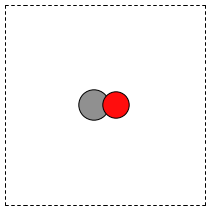
\includegraphics[width=2in]{./images/simple-cubic-cell.png}



\subsection{Using in-built databases}
\label{sec-4-2}

We can load predefined molecules from \verb~ase.structure.molecule~. For example, the database contains the molecules in the G2 set (\url{http://www.cse.anl.gov/OldCHMwebsiteContent/compmat/comptherm.htm}) among others. These are generally the result of MP2/6-31g(d) calculations from a code like \texttt{GAUSSIAN} or \texttt{GAMESS}. Consequently, they will not have unit cell information, and will have a default unit cell of  (( 1.  0.  0.), ( 0.  1.  0.), ( 0.  0.  1.)). We need to manually specify the unit cell for a \texttt{VASP} calculation.

\begin{minted}[frame=lines,fontsize=\scriptsize,linenos]{python}
from ase.structure import molecule
from ase.visualize import view

atoms = molecule('CO')

view(atoms)
print atoms
print 'Old Cell:'
print atoms.get_cell()

atoms.set_cell((10,10,10), scale_atoms=False)
print 'New Cell:'
print atoms.get_cell()
view(atoms)
\end{minted}

The g2 set as implemented in ase is given below.

\begin{verbatim}
isobutene                CH3CH2OH                 CH3COOH
COF2                     CH3NO2                   CF3CN
CH3OH                    CCH                      CH3CH2NH2
PH3                      Si2H6                    O3
O2                       BCl3                     CH2_s1A1d
Be                       H2CCl2                   C3H9C
C3H9N                    CH3CH2OCH3               BF3
CH3                      CH4                      S2
C2H6CHOH                 SiH2_s1A1d               H3CNH2
CH3O                     H                        BeH
P                        C3H4_C3v                 C2F4
OH                       methylenecyclopropane    F2O
SiCl4                    HCF3                     HCCl3
C3H7                     CH3CH2O                  AlF3
CH2NHCH2                 SiH2_s3B1d               H2CF2
SiF4                     H2CCO                    PH2
OCS                      HF                       NO2
SH2                      C3H4_C2v                 H2O2
CH3CH2Cl                 isobutane                CH3COF
HCOOH                    CH3ONO                   C5H8
2-butyne                 SH                       NF3
HOCl                     CS2                      P2
C                        CH3S                     O
C4H4S                    S                        C3H7Cl
H2CCHCl                  C2H6                     CH3CHO
C2H4                     HCN                      C2H2
C2Cl4                    bicyclobutane            H2
C6H6                     N2H4                     C4H4NH
H2CCHCN                  H2CCHF                   cyclobutane
HCl                      CH3OCH3                  Li2
Na                       CH3SiH3                  NaCl
CH3CH2SH                 OCHCHO                   SiH4
C2H5                     SiH3                     NH
ClO                      AlCl3                    CCl4
NO                       C2H3                     ClF
HCO                      CH3CONH2                 CH2SCH2
CH3COCH3                 C3H4_D2d                 CH
CO                       CN                       F
CH3COCl                  N                        CH3Cl
Si                       C3H8                     CS
N2                       Cl2                      NCCN
F2                       CO2                      Cl
CH2OCH2                  H2O                      CH3CO
SO                       HCOOCH3                  butadiene
ClF3                     Li                       PF3
B                        CH3SH                    CF4
C3H6_Cs                  C2H6NH                   N2O
LiF                      H2COH                    cyclobutene
LiH                      SiO                      Si2
C2H6SO                   C5H5N                    trans-butane
Na2                      C4H4O                    SO2
NH3                      NH2                      CH2_s3B1d
ClNO                     C3H6_D3h                 Al
CH3SCH3                  H2CO                     CH3CN
\end{verbatim}


\subsection{Reading structures from files}
\label{sec-4-3}

ASE can read a variety of data formats using \verb~ase.io.read~. For example, here is a cif file I downloaded from \url{http://materialsproject.org}.

\url{mp-22862_NaCl.cif}

\begin{minted}[frame=lines,fontsize=\scriptsize,linenos]{python}
from ase.io import read
from ase.visualize import view

atoms = read('mp-22862_NaCl.cif')

view(atoms)
print atoms
\end{minted}

\begin{verbatim}
Atoms(symbols='Na4Cl4', positions=..., cell=[[5.69169356, 0.0, 0.0], [3.485157149990802e-16, 5.69169356, 0.0], [3.485157149990802e-16, 3.485157149990802e-16, 5.69169356]], pbc=[True, True, True])
\end{verbatim}



\section{Simple SCF calculations}
\label{sec-5}

We will now perform a simple calculation on our CO molecule. This is done by creating a \texttt{jasp} calculator, which is an extension of the default Vasp calculator in ase (\verb~ase.calculators.vasp~). The two properties that we will calculate in this example are the energy and the forces on the atoms. 

The first time we run this code, a calculation will be submitted to the Notre Dame queue system. So when you try to print the potential energy of you will get an exception saying VaspSubmitted. You can check the status of the job by going back to the terminal and typing \verb~qstat -u netid~. Once the job has finished running you can rerun the code, and if all went well, it should give you the energies and the forces.

\begin{minted}[frame=lines,fontsize=\scriptsize,linenos]{python}
from ase import Atoms, Atom
from ase.io import write
from ase.visualize import view
from jasp import jasp

JASPRC['queue.q'] = 'long'
JASPRC['queue.nprocs'] = 8
JASPRC['queue.pe'] = '*@@schneider'

# define an Atoms object
co = Atoms([Atom('C', [0., 0., 0.]),
            Atom('O', [1.1, 0., 0.])],
           cell=(10, 10, 10))

with jasp('molecules/simple-co',  # output dir relative to current dir
          xc='PBE',  # the exchange-correlation functional
          nbands=8,    # number of bands
          encut=350,    # planewave cutoff
          ismear=1,    # Methfessel-Paxton smearing
          sigma=0.01,  # very small smearing factor for a molecule
          atoms=co) as calc:
    print('energy = {0} eV'.format(co.get_potential_energy()))
    print 'Forces (eV/Ang.):'
    print(co.get_forces())
    print 'SCF iterations = {0}'.format(calc.get_number_of_iterations())
    print calc # Prints a summary of the calculation
    #Note: some properties are attributes of the atoms object and some of the calc.
\end{minted}

\begin{verbatim}
energy = -14.69232797 eV
Forces (eV/Ang.):
[[-5.777  0.     0.   ]
 [ 5.777  0.     0.   ]]
SCF iterations = 16
: -----------------------------
  VASP calculation from /afs/crc.nd.edu/user/p/pmehta1/computational-chemistry/Lab3/molecules/simple-co
  converged: True
  Energy = -14.692328 eV

  Unit cell vectors (angstroms)
        x       y     z      length
  a0 [ 10.000  0.000  0.000] 10.000
  a1 [ 0.000  10.000  0.000] 10.000
  a2 [ 0.000  0.000  10.000] 10.000
  a,b,c,alpha,beta,gamma (deg):10.000 10.000 10.000 90.0 90.0 90.0
  Unit cell volume = 1000.000 Ang^3
  Stress (GPa):xx,   yy,    zz,    yz,    xz,    xy
            -0.004  0.002  0.002-0.000 -0.000 -0.000
 Atom#  sym       position [x,y,z]tag  rmsForce constraints
   0    C   [0.000      0.000      0.000]  0   5.78      T T T
   1    O   [1.100      0.000      0.000]  0   5.78      T T T
--------------------------------------------------

INCAR Parameters:
-----------------
        nbands: 8
        ismear: 1
         encut: 350.0
         sigma: 0.01
        magmom: None
          kpts: [1, 1, 1]
    reciprocal: False
            xc: PBE
           txt: -
         gamma: False

Pseudopotentials used:
----------------------
C: potpaw_PBE/C/POTCAR (git-hash: ee4d8576584f8e9f32e90853a0cbf9d4a9297330)
O: potpaw_PBE/O/POTCAR (git-hash: 592f34096943a6f30db8749d13efca516d75ec55)
\end{verbatim}

We can also look at the files created by \texttt{VASP} to see if everything went ok. 



\section{Geometry Optimizations}
\label{sec-6}

Now let us try to do a geometry optimization. For this \texttt{VASP} needs two additional keywords (at least) - \verb~IBRION~ and \verb~NSW~. \verb~IBRION~ controls the relaxation algorithm and \verb~NSW~ specifies the total number of steps.

\begin{minted}[frame=lines,fontsize=\scriptsize,linenos]{python}
from ase import Atoms, Atom
from ase.io import write
from ase.visualize import view
from jasp import jasp

# define an Atoms object
co = Atoms([Atom('C', [0., 0., 0.]),
               Atom('O', [1.1, 0., 0.])],
              cell=(10, 10, 10))

with jasp('molecules/geometry-co',  # output dir relative to current dir
          xc='PBE',  # the exchange-correlation functional
          nbands=8,    # number of bands
          encut=350,    # planewave cutoff
          ismear=1,    # Methfessel-Paxton smearing
          sigma=0.01,  # very small smearing factor for a molecule
          nsw=20, # Number of ionic steps
          ibrion=2, # Conjugate gradient alogrithm
          atoms=co) as calc:
    print('energy = {0} eV'.format(co.get_potential_energy()))
    print 'Forces (eV/Ang.):'
    print(co.get_forces())
    print 'Equilibrium Positions (Angs.):'
    for atom in co:
        print atom.symbol, atom.position
    
# Save an image. Note that this is done outside the with statement
write('images/CO-relaxed.png', co, show_unit_cell=2, rotation='60x,-30y,90z')
\end{minted}

\begin{verbatim}
energy = -14.81175954 eV
Forces (eV/Ang.):
[[ 0.003  0.     0.   ]
 [-0.003  0.     0.   ]]
Equilibrium Positions (Angs.):
C [-0.022  0.     0.   ]
O [ 1.122  0.     0.   ]
\end{verbatim}

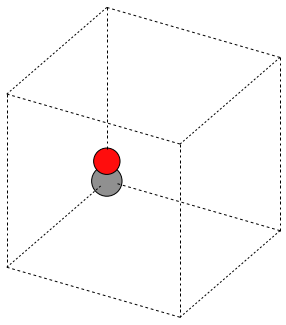
\includegraphics[width=2in]{./images/CO-relaxed.png}


We might also want to visualize the relaxation trajectory. Using the terminal, change into the directory where you performed the calculation, and type in \verb~jaspsum -t~.


\section{Effect of Unit Cell Size}
\label{sec-7}

Let us consider a more complicated example. Here we will vary the size of the unit cell, to see how interactions between periodic images affect the energy.

\begin{minted}[frame=lines,fontsize=\scriptsize,linenos]{python}
from jasp import *
from ase import Atoms,Atom
import numpy as np

atoms = Atoms([Atom('C',[0,   0, 0]),
               Atom('O',[1.2, 0, 0])])

L = [4, 5, 6, 8, 10]

energies = []

ready = True

for a in L:
    atoms.set_cell([a,a,a], scale_atoms=False)
    atoms.center()
    with jasp('molecules/co-L-{0}'.format(a),
              encut=350,
              xc='PBE',
              atoms=atoms) as calc:
        try:
            energies.append(atoms.get_potential_energy())
        except (VaspSubmitted, VaspQueued):
            ready = False

if not ready:
    import sys; sys.exit()

import matplotlib.pyplot as plt
plt.plot(L, energies, 'bo-')
plt.xlabel('Unit cell length ($\AA$)')
plt.ylabel('Total energy (eV)')
plt.savefig('images/co-e-v.png')
plt.show()
\end{minted}

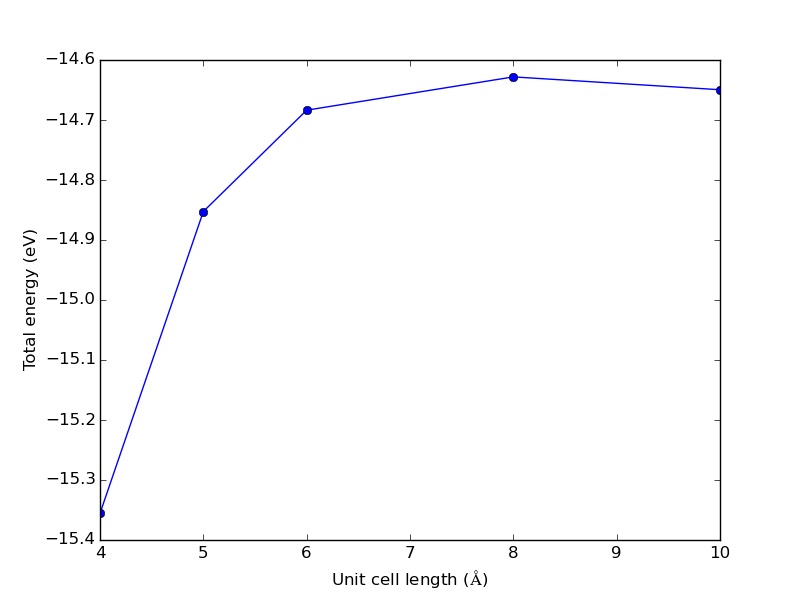
\includegraphics[width=.9\linewidth]{./images/co-e-v.png}


We can see that at small box sizes, there are attractive interactions between CO molecules that lower the total energy. At larger box sizes the energy starts to converge to a fixed value as the interactions are minimized. Now let's check the effect on the computational cost.

\begin{minted}[frame=lines,fontsize=\scriptsize,linenos]{python}
from jasp import *

L = [4, 5, 6, 8, 10]

for a in L:
    with jasp('molecules/co-L-{0}'.format(a)) as calc:
        print '{0} {1} seconds'.format(a, calc.get_elapsed_time())
\end{minted}

\begin{verbatim}
4 2.616 seconds
5 3.907 seconds
6 5.891 seconds
8 16.588 seconds
10 30.543 seconds
\end{verbatim}

We can see the computational cost went up by a factor of 15! Perhaps you can now appreciate the computational cost involved in simulating 100s of atoms in large boxes!




\section{Miscellaneous}
\label{sec-8}

\subsection{Building pdfs from org files}
\label{sec-8-1}

Using the software you loaded at the beginning of lab, you should be able to build a pdf from your .org files. Let us try that, click on the Org menu and click Export/Publish. Then press 'l' and 'o'. This let's you build a pdf and open it.

Alternately, you can type, \verb~C-c C-e l o~


\subsection{Viewing latex equations in org documents}
\label{sec-8-2}

Click on \url{org-toggle-latex-overlays}. You should be able to see the Schrodinger equation below.

\begin{itemize}
\item $H\psi = E\psi$
\end{itemize}
% Emacs 24.4.3 (Org mode 8.2.10)
\end{document}